% ch1.tex
% This work is licensed under the Creative Commons Attribution-Noncommercial-Share Alike 3.0 New Zealand License.
% To view a copy of this license, visit http://creativecommons.org/licenses/by-nc-sa/3.0/nz
% or send a letter to Creative Commons, 171 Second Street, Suite 300, San Francisco, California, 94105, USA.


\chapter{Nem todas cobras te morderão}\label{ch:notallsnakeswillsquishyou}

Há possibilidade de que este livro tenha sido lhe dado em seu aniversário, ou possivelmente no Natal. Tia Amélia lhe daria um par de meias duas vezes maior que o seu pé (e que mesmo se servisse, você não gostaria de usar). Mas ao invés disso, ela ouviu alguém falando sobre a versão impressa deste livro e logo lembrou que você tinha um daqueles compu-alguma-coisa, que inclusive tentou ensiná-la a usar uma vez, no último Natal (até que ela começasse a tentar falar com o mouse), e pediu-lhe para que imprimisse mais uma cópia. Seja grato por não ter ganho aquele velho par de meias.

Espero que você não esteja tão decepcionado, por eu surgir de um papel de presentes reciclado, ao invés disso. Um não-tão-falante (ok, um nada-falante) livro, com um título aparentemente ameaçador na capa ``Aprendendo$\ldots$''.
Mas espere um momento para pensar em como eu me sinto. Se você fosse o personagem daquela novela sobre magos que estão na prateleira de livros do seu quarto, eu possivelmente teria dentes… ou até olhos. Eu poderia mover figuras dentro de mim, ou ser capaz de fazer sons fantasmagóricos enquanto você folheia minhas páginas. Mas pelo contrário, eu sou impresso em folhas de papel A4 com algumas orelhas, ou quem sabe grampeados, dentro de uma pasta. Como eu saberia---Eu não tenho olhos.
\\
\\
\emph{Eu daria qualquer coisa por alguns belos e afiados dentes$\ldots$}
\\
\\
Porém isso não é tão ruim quanto parece. Mesmo que eu não possa falar... ou morder os seus dedos enquanto não está olhando... Eu posso lhe dizer um pouquinho como os computadores funcionam. Nada da parte física, com fios, chips, cabos e outros dispositivos que, mais do que provável, lhe dariam choque antes mesmo que o tocassem (então, não!!)---mas as coisas escondidas que rodam entre esses fios, chips de computador, cabos e bits, que fazem o seu computador ter alguma utilidade.

\begin{wrapfigure}{r}{0.5\textwidth}
  \begin{center}
\includegraphics*[width=70mm]{eps/electrocute.eps}
  \end{center}
\end{wrapfigure}

É um pouco como os pensamentos rodando dentro da sua cabeça. Se você não tivesse pensamentos, você estaria sentado no chão do seu quarto, olhando vagarosamente para a porta e babando sobre a sua camiseta. Sem os \emph{programas}, os computadores serviriam apenas para apoiar portas---e mesmo assim ainda não seriam muito úteis, pois você ainda tropeçaria sobre eles durante a noite. E convenhamos que, não há nada pior que tropeçar no escuro e bater o dedinho do pé.
\\
\\
\emph{Eu sou apenas um livro e eu sei disso.}
\\
\\
Sua família pode ter um Playstation, Xbox ou Wii na sala----eles não teriam muito uso sem os programas (jogos) para fazê-los funcionar. Seu aparelho de DVD, possivelmente sua geladeira e seu carro, todos usam programas de computador que os tornam mais prestativos do que seriam. Seu aparelho de DVD tem programas que ajudam-o a escolher o que quer assistir no DVD; sua geladeira pode ter um simples programa que o ajuda a economizar energia elétrica, e mesmo assim mantém a comida conservada; seu carro pode ter um computador, que possui um programa, que alerta o motorista sobre uma possível colisão.\\
Se você souber como escrever programas de computador, você pode fazer todos tipos de coisas úteis. Quem sabe escrever seus próprios jogos. Criar web sites que realmente façam algo, não apenas deixá-los com um visual colorido. Ser capaz de programar o ajudaria até com o seu dever de casa.\\
\\
Como dito, vamos para algo um pouco mais interessante.

\section{Um pouco sobre linguagens}

Assim como os humanos, certamente as baleias, possivelmente os golfinhos, e talvez alguns pais (embora isso seja discutível), computadores tem sua própria linguagem. Atualmente, como os humanos, eles tem até mais de uma linguagem. Praticamente há uma linguagem para cada letra do alfabeto. A, B, C, D e E não são apenas letras, mas também linguagens de programação (que provam que adultos não tem imaginação, e deveriam ter lido um dicionário, ou ao menos uma enciclopédia, antes de nomear algo).

Há linguagens de programação com nomes de pessoas, nomeadas usando simples acrônimos (a primeira letra de uma série de palavras), e apenas algumas nomeadas após um programa de TV. Ah, e se você adicionar alguns sinais de adição, ou sustenidos (+, \#) após algumas das letras que mencionei---você terá mais algumas linguagens de programação. Tornando as coisas piores, algumas linguagens de programação são praticamente a mesma coisa, diferenciando-se levemente.
\\
\\
\emph{O que eu te disse?  Sem imaginação!}
\\
\\
Felizmente, muitas dessas linguagens caíram em desuso, ou sumiram completamente; mas a lista de diferentes formas que você pode `falar' com o computador continua preocupantemente grande. Irei discutir apenas uma delas--caso contrário nem mesmo teriamos começado.
\\
Seria mais produtivo sentar-se em seu quarto e babar sobre a sua camiseta$\ldots$

\section{A Ordem das Não-venenosas \\Serpentes Constritoras$\ldots$}

$\ldots$ou Pythons (Pítons em português), mais especificamente.

Além de ser uma cobra, Python\index{Python} também é uma linguagem de programação. Porém, não foi nomeada com o nome de um réptil sem patas; mas é uma das linguagens de programação nomeadas após um programa de TV. Monty Python foi um popular programa humorístico de TV britânico, durante a década de 70 (e continua popular até hoje), que você deve ter uma certa idade para achar engraçado. Qualquer um abaixo dessa idade$\ldots$ digamos 12$\ldots$ ficará se perguntando do que se trata\footnote{Exceto a dança-do-peixe-na-cara. Que é engraçado independente da sua idade.}.

Existe uma série de coisas sobre Python (a linguagem de programação, não a cobra, nem o programa de TV) que a fazem extremamente útil quando você está aprendendo a programar. Para nós, no momento, o motivo mais importante é que você pode começar a fazer as coisas muito mais rapidamente.

Esta é a parte em que você espera que a sua Mãe, Pai (ou quem estiver responsável pelo computador), tenha lido o começo do livro, rotulado ``Um recado aos Pais''.

\noindent
Existe um bom modo de saber se eles realmente leram:

\begin{WINDOWS}
Clique no botão `Iniciar' no canto inferior esquerdo da tela, e vá em `Todos programas' (que tem um triangulo verde ao lado), e espera-se que na lista de programas você veja `Python 3.2' (ou algo parecido). Figura~\ref{fig1} mostra o que você deve visualizar. Clique em `Python (command line)' como mostrado na Figura~\ref{fig1}.

\begin{figure}
\begin{center}
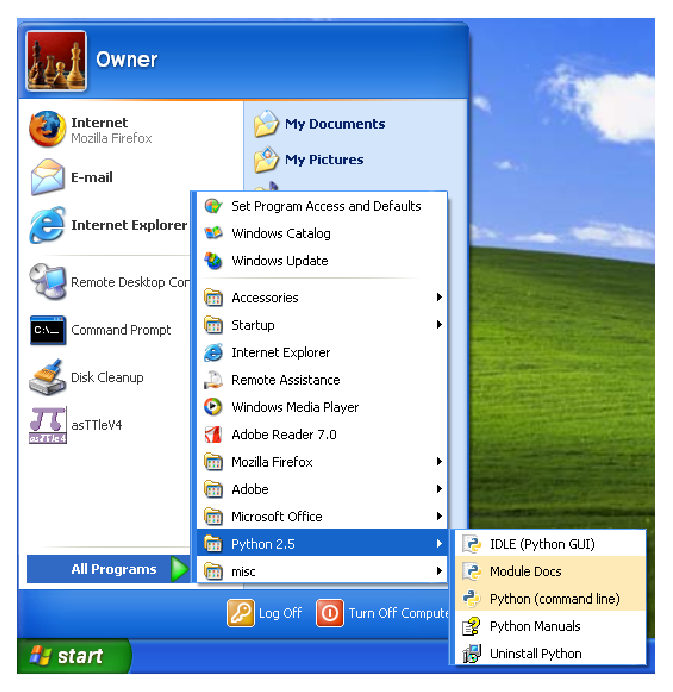
\includegraphics[width=80mm]{eps/figure1.eps}
\end{center}
\caption{Python no menu do Windows.}\label{fig1}
\end{figure}

\begin{figure}
\begin{center}
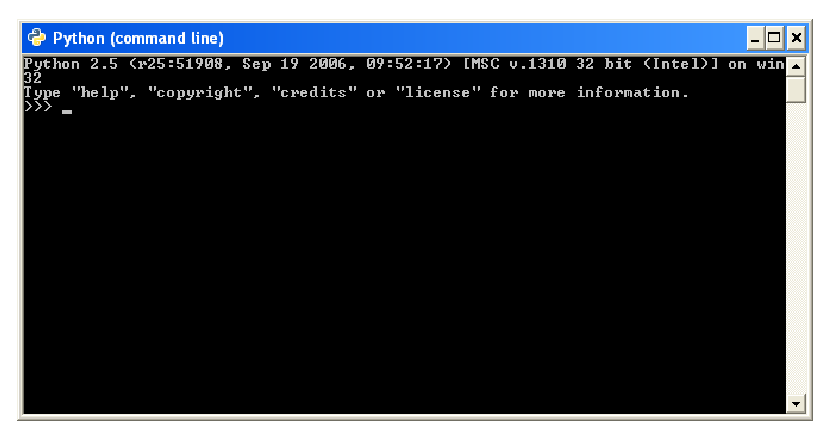
\includegraphics[width=135mm]{eps/figure2.eps}
\end{center}
\caption{Interpretador Python no Windows.}\label{fig2}
\end{figure}
\end{WINDOWS}

\begin{MAC}
Na barra lateral do Finder, você deve ver um grupo chamado `Aplicativos'. Clique sobre ele, e então procure pelo programa chamado `Terminal' (provavelmente estará dentro da pasta `Utilitários').
Clique em `Terminal', e quando abrir, digite python e pressione enter. Esperamos que você veja uma tela parecida com a Figura~\ref{fig3}.

\begin{figure}
\begin{center}
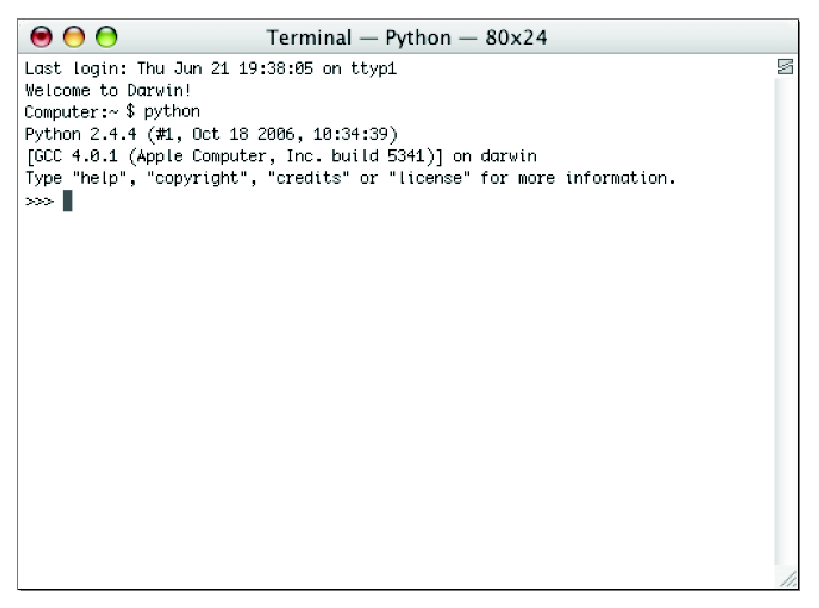
\includegraphics[width=85mm]{eps/figure3.eps}
\end{center}
\caption{Interpretador Python no Mac OSX.}\label{fig3}
\end{figure}
\end{MAC}

\begin{LINUX}
Pergunte a Mãe ou Pai qual programa de terminal utilizar (pode se chamar `Konsole', `rxvt', `xterm' ou qualquer um dos programas disponíveis---que é o motivo pelo qual você provavelmente precisará perguntar). Inicie o terminal e digite `python' (sem as aspas), e pressione enter. Você verá algo como na Figura~\ref{fig4}.

\begin{figure}
\begin{center}
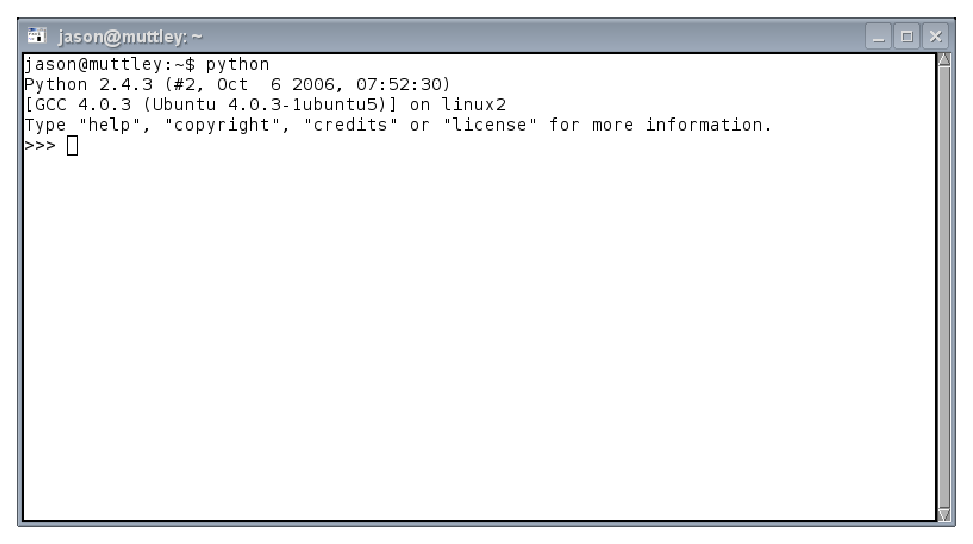
\includegraphics[width=80mm]{eps/figure4.eps}
\end{center}
\caption{Interpretador Python no Linux.}\label{fig4}
\end{figure}
\end{LINUX}

\subsection*{\color{BrickRed}Se você descobrir que eles não leram o começo do livro$\ldots$}

$\ldots$porque está faltando algo quando você tenta seguir essas instruções---então vire a página até o começo do livro e coloque-o sobre o jornal que eles estão tentando ler, olhando-os com confiança. Dizendo, ``por favor, por favor'' de novo e de novo, até que se torne chato o bastante, deve funcionar bem, caso você esteja tendo problemas para tirá-los do sofá. E claro, uma outra alternativa, é você tentar seguir as instruções da `Introdução', de como instalar o Python, você mesmo.

\section{Seu primeiro programa em Python}

Com sorte, se você chegou até aqui, você já deve ter iniciado o Interpretador Python, que é uma das formas de executar comandos e programas em Python. Quando você o inicia pela primeira vez (ou após executar algum comando), você verá o que chamamos de `prompt'. No Interpretador Python\index{Interpretador Python}, o `prompt' é indicado por três sinais de `maior que' ($>$):

\begin{listing}
\begin{verbatim}
>>>
\end{verbatim}
\end{listing}

Se você juntar alguns comandos Python necessários, você terá um programa que poderá rodar não apenas no interpretador$\ldots$ mas no momento, nós queremos deixar as coisas simples, digitando nossos comandos diretamente no interpretador, no `prompt' ($>>>$). Então, por que não começamos digitando o seguinte:

\begin{listing}
\begin{verbatim}
print("Ola mundo")
\end{verbatim}
\end{listing}

Certifique-se de colocar as aspas (que são essas: $"$ $"$), e pressionar a tecla `enter' no final da linha. Esperando que você veja algo parecido com isso:

\begin{listing}
\begin{verbatim}
>>> print("Ola mundo")
Ola mundo
\end{verbatim}
\end{listing}

O `prompt' reaparece, informando-o que o Interpretador Python já está pronto para outros comandos.

\noindent
Parabéns! Você acaba de criar seu primeiro programa em Python. \code{print} é a função que escreve no interpretador, o que estiver entre os parênteses---em breve, nós o utilizaremos novamente.

\section{Seu segundo programa em Python$\ldots$o mesmo?}

Os programas em Python não seriam tão úteis assim, caso você tivesse que digitar cada comando, toda hora que quisesse fazer algo---ou se você escrevesse um programa para alguém, e ele tivesse que digitar tudo de novo, antes de usá-lo.

O editor de texto que você utiliza para fazer seus trabalhos de escola, deve ter em torno de 10 a 100 milhões de linhas de código. Dependendo do número de linhas que você imprimir por página (imprimindo ou não em frente e verso), isso daria por volta de 400,000 páginas$\ldots$ ou uma pilha de papel de mais de 40 metros.
Imagine que, quando você levasse esse programa da loja para a sua casa, você teria que fazer várias viagens de ida e volta, para carregar tanto papel$\ldots$

$\ldots$e ainda teria que torcer para não ocorresse nenhuma rajada de vento, enquanto carregava os papéis. Felizmente, há uma alternativa para tudo que foi dito aqui---ou ninguém faria nada disso.

\begin{center}
\includegraphics*[width=85mm]{eps/pullinghair.eps}
\end{center}

\begin{WINDOWS}
Abra o Bloco de notas (Clique em Iniciar, Todos Programas, e em Acessórios), e então digite o comando \code{print}, exatamente como você digitou anteriormente no interpretador:

\begin{listing}
\begin{verbatim}
print("Ola mundo")
\end{verbatim}
\end{listing}

Clique no menu Arquivo (no Bloco de notas) e salve-o na Área de Trabalho com o nome \emph{ola.py}. Clique duas vezes sobre o ícone do \emph{ola.py} na sua Área de Trabalho (veja a Figura~\ref{fig5}) e então aparecerá, muito rapidamente, a janela do Interpretador Python. Que desaparecerá muito rapidamente também, antes mesmo que você consiga ler o que está escrito, mas a frase `Ola mundo' deve aparecer na tela por uma fração de segundo---nós voltaremos nisso em breve e provaremos que isso realmente ocorreu.\\

\begin{figure}
\begin{center}
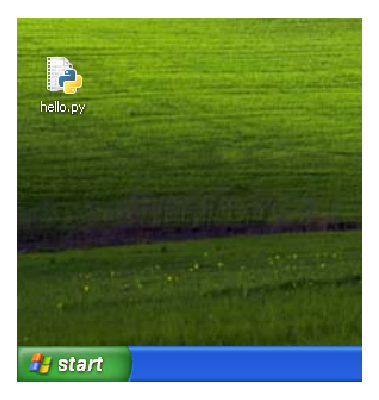
\includegraphics[width=58mm]{eps/figure5.eps}
\end{center}
\caption{Ícone do ola.py na Área de Trabalho.}\label{fig5}
\end{figure}
\end{WINDOWS}

\begin{MAC}
Abra o seu Editor de Texto clicando sobre o seu ícone. Pode estar no Dock, na parte inferior da tela \includegraphics*[width=12mm]{eps/textedit-icon.eps}, ou procure pelo ícone \includegraphics*[width=19mm]{eps/textedit-icon2.eps} na lista de Aplicativos, no Finder. Digite o comando \code{print} exatamente como você digitou anteriormente no interpretador:

\begin{listing}
\begin{verbatim}
print("Ola mundo")
\end{verbatim}
\end{listing}

Clique no menu Arquivo e salve-o no seu diretório (barra lateral esquerda do Finder, em Locais---pergunte a sua Mãe ou Pai caso não ache) com o nome \emph{ola.py}.

Abra o `Terminal' novamente---ele abrirá automaticamente no seu diretório---e siga as instruções:

\begin{listing}
\begin{verbatim}
python ola.py
\end{verbatim}
\end{listing}

Você deverá ver a frase `Ola mundo' exatamente como você digitou no Interpretador Python.

\end{MAC}

\begin{LINUX}
Abra o editor de texto (pergunte a sua Mãe ou Pai qual utilizar), e então digite o comando \code{print}, exatamente como você digitou anteriormente no interpretador:

\begin{listing}
\begin{verbatim}
print("Ola mundo")
\end{verbatim}
\end{listing}

Clique no menu Arquivo, salve-o no seu diretório pessoal (deve ter um ícone chamado Pasta Pessoal, em algum lugar da janela Salvar). Após isso, abra o terminal (Konsole, rxvt, etc... o que você usou anteriormente), e digite:

\begin{listing}
\begin{verbatim}
python ola.py
\end{verbatim}
\end{listing}

Você deverá ver a frase `Ola mundo' exatamente como digitou no Interpretador Python. (veja a Figura~\ref{fig9}).

\begin{figure}
\begin{center}
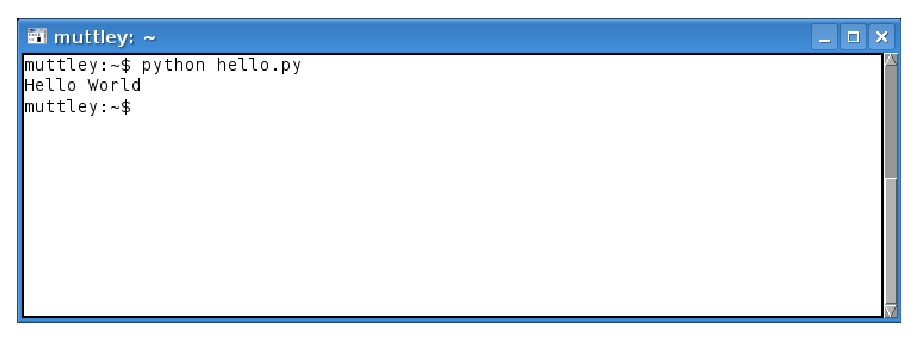
\includegraphics[width=75mm]{eps/figure9.eps}
\end{center}
\caption{Executando um programa Python a partir de um arquivo texto, no Linux.}\label{fig9}
\end{figure}
\end{LINUX}

Agora você pode ver que as boas pessoas que criaram o Python, amavelmente, salvaram-o de ter que digitar a mesma coisa repetidas e repetidas vezes. Como fizeram alguns lá nos anos 80. É sério---eles fizeram. Vá e pergunte ao seu pai, se ele já não teve um \emph{ZX81} quando era criança.\\

\noindent
Se já teve, você pode apontar para ele e começar a rir.\\

\noindent
Acredite em mim. Você não vai entender isso, mas ele vai.\footnote{O Sinclair ZX81, lançado nos anos 80, foi um dos primeiros computadores pessoais acessíveis. Uma série de jovens, garotos e garotas, ficaram enlouquecidos, digitando o código de alguns jogos que vinham nas populares revistas sobre o ZX81---descobrindo somente após horas de digitação, que aquelas maluquices jamais funcionaram como deveriam.}

\noindent
\emph{Porém esteja preparado para correr.}

\subsection*{\color{BrickRed}O fim do começo}

Bem-vindo ao maravilhoso mundo da Programação. Nós começamos com um simples programa de ``Ola mundo''---todo mundo começa assim quando estão aprendendo a programar.
No próximo capítulo, nós começaremos a fazer coisas mais úteis com o Interpretador Python, e veremos como são feitos os programas.

\newpage
